% !TEX root = paper.tex
\section{Evaluation}

We evaluate both the tracking system and the calibration to quantize the tracking error and locate the main sources of inaccuracies.
%\lipsum[1] % Dummy text

\subsection{Evaluation of Tracking [SE]}

As we used a closed form solution for the inverse kinematics, the robot movements itself can be seen as accurate. 
The main source for errors is therefore, apart from imperfect hand-eye calibration, the head tracking. To evaluate the accuracy of the head tracking, we mounted the head on the UR5 and used the touch panel to move it accurately along each axes. 
As the coordinate systems of the UR5 and the camera did not align, we only considered relative movement based on the standing head at the beginning of each measurement. We expected the head tracking result to vary in a small intervall around the actual value while the robot was not moving. For a moving head we expected that the tracking would lag behind but reach the correct final value. 

These assumptions were confirmed in many of the measurements. As expected, lower speeds  delivered in general better results. For some movements we experienced that the tracking system could not catch up with the robot. After the completion of the movement, a static error remained. Figure \ref{fig:z70} displays this behavior. The upper plot shows the actual movement in blue and the predicted movement in orange. The lower plot shows the absolute error, so the differences between both curves. 

\begin{figure}[ht]
    \centering
    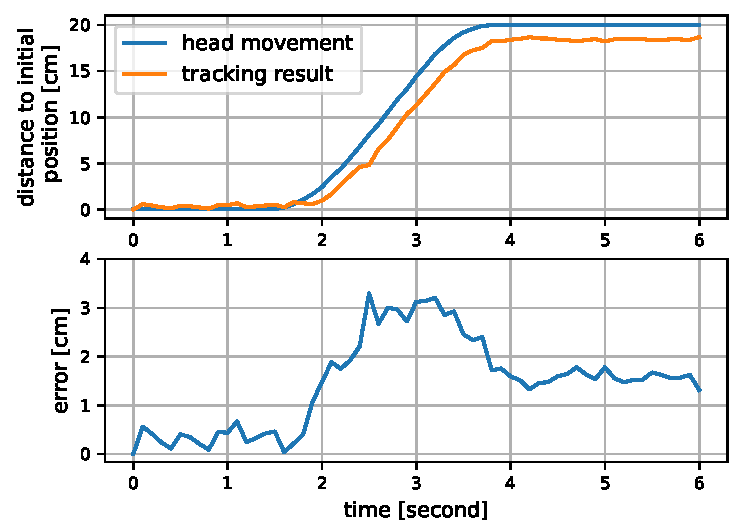
\includegraphics[width=\linewidth]{tracking_eval_z70}
    \caption{Movement along Robot z axes, 70\% speeds}
    \label{fig:z70}
\end{figure}

The best results were achieved for movements in robot $y$ axes. Even at 100\% speed we got surprisingly low errors. A reason for that might be, that nearly all the complete movement in that direction took place towards or away from the camera. Therefore the movement could be well identified by the IR depth sensor. Figure \ref{fig:y100} shows the measurements for that case. 


\begin{figure}[ht]
    \centering
    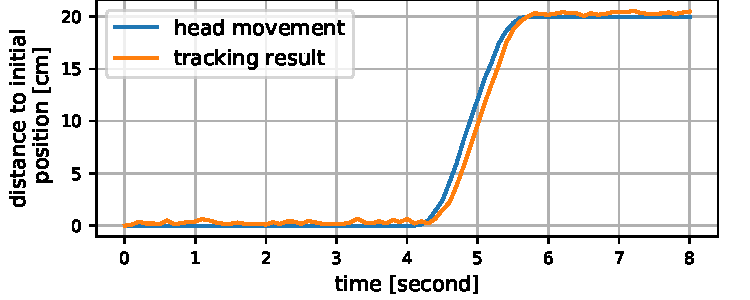
\includegraphics[width=\linewidth]{tracking_eval_y100_single}
    \caption{Movement along Robot y axes, 100\% speeds}
    \label{fig:y100}
\end{figure}

Table \ref{tab:rmse} shows the root-mean-square error (RMSE) for each measurement. A control measurement with a not moving head resulted in a RMSE of 0.069 cm. The extremely high error for axes x at 100\% speed is likely to be caused by some error in the test setup and not part of the normal performance of our system. Due to the limited time with the robot, we were not able to additional testing to confirm or refute this value. 


\begin{table}[hbt]
    \caption{RMSE [cm] of head tracking}
    \centering
    \begin{tabular}{l|cccc}
        \toprule
        & \multicolumn{4}{c}{speed [\%]} \\
        Axes & 30 & 50 & 70 & 100 \\
        \midrule
        x & 1.789 & 0.880 & 1.671 & 4.701 \\
        y & 0.431 & 0.614 & 0.736 & 0.801 \\
        z & 0.453 & 0.482 & 1.744 & 1.863 \\
        \bottomrule
    \end{tabular}
    \label{tab:rmse}
\end{table}

The big differences for the different axes suggest that intelligent placement of the camera is very important. The camera should if possible be placed in line with the biggest expected movement.  

\subsection{Accuracy of Hand-Eye Calibration [PV]}

From equation \eqref{eqn:HandEye} it is easy to see that the transformation from robot base to its own base in a loop (through M,N,X,Y) is identity. This fact is taken as a measure of the quality of the hand eye calibration. The RMS value of the positional error for the 10 poses that are far apart from each were calculated and standard deviation of these 10 RMS values is $\sigma = 0.00329$. There is a scope to improve the handeye calibration accuracy.  

%\lipsum[1] % Dummy text

%\lipsum[1] % Dummy text
